% !TeX spellcheck = fr-moderne
\section{Introduction de l'industrie de la télécommunication}
\subsection{L'evolution des normes de téléphonie mobile}
Depuis 1984, il y a déjà plusieurs standards ont été utilisé par les opérateur dans le monde entier. Voici un tableau de différentes standards mobile en Europe et ses paramétrés \ref{tbl:GMIE}. 
\begin{table}[H]
\begin{tabular}{|p{2cm}|p{2cm}|p{2cm}|p{4cm}|}
	\hline
	Génération&Acronyme&Description&Débit\\
	\hline
	1G		&Radiocom 2000	&Échanges de type voix uniquement&analogique\\
	\hline
	\hline
	2G		&GSM			&Échanges de type voix uniquement	&9,05 kbps\\
	\hline
	2,5G	&GPRS			&Échange de données sauf voix		&171,2 kbps / 50 kbps / 17,9 kbps\\
	\hline
	\hline
	3G		&UMTS			&Voix + données						&144 kbps rurale, 384 kbps urbaine, 1,9 Mbps point fixe / -\\
	\hline
	3.5G ou 3G+ ou H&HSPA	&Évolution de l'UMTS				&14,4 Mbps / 3,6 Mbps / -\\
	\hline
	\hline
	4G		&LTE			&Long Term Evolution (Données)				&150 Mbps / 40 Mbps / -\\
	\hline
	4G		&LTE-Advanced	&Long Term Evolution Advanced (Données+voix)		&1 Gbps à l'arrêt, 100 Mbps en mouvement / - / -\\
	\hline
\end{tabular}
\caption{Les différentes générations de téléphonie mobile en Europe}
 \label{tbl:GMIE}
\end{table}

\subsubsection{La premier génération}
En télécommunication, \textsf{1G} est la premier génération des standards pour la téléphonie mobile, il s'agit de la première apparition du réseaux de téléphonie mobile, 1G sont des réseaux analogiques, peut échanges de type voix uniquement.
\subsubsection{La deuxième génération}
\textsf{2G}, la technologie de téléphonie sans fil de deuxième génération, la différence entre le réseaux 1G et 2G est: le signaux radio sur les réseaux 1G sont analogiques, et celle de 2G sont numériques.

Systèmes 2G ont été significativement plus efficaces du spectre permettant de bien plus grand taux de pénétration du téléphone mobile, en plus les données vocales numériques peuvent être compressées et multiplexées beaucoup plus efficacement que les codages de la voix analogique grâce à l'utilisation de codecs différents, ce qui permet plus d'appels à transmettre dans la même quantité de bande passante radio. Et 2G présenté premier foi le service de données pour mobile. Les Technologie 2G permettent les divers réseaux de téléphonie mobile de utiliser des services tels que le SMS et MMS. Tous les message de texte envoyés au delà de 2G sont chiffrés numériquement, ce qui permet le transfert de données de telle sorte que seul le destinataire peut recevoir et lire.   

Réseaux 2G ont été construits principalement pour le service téléphoniques et de transmission de données lent (défini dans les documents de spécifications IMT-2000).

Réseaux \textsf{2,5G}, on le qualifie souvent de le General packet Radio Service ou GPRS, est une norme pour la téléphonie mobile dérivée du GSM et complémentaire de celui-ci, permettant un débit de données plus élevé. Le 2,5 indique que c'est une technologie à mi-chemin entre le GSM (deuxième génération) et l'UMTS (troisième génération). Le GPRS est une extension du protocole GSM : il ajoute par rapport à ce dernier la transmission par paquets. Cette méthode est plus adaptée à la transmission des données. En effet, les ressources ne sont allouées que lorsque des données sont échangées, contrairement au mode « circuit » en GSM où un circuit est établi – et les ressources associées – pour toute la durée de la communication. Le GPRS a ensuite évolué au début des années 2000 vers la norme \textsc{edge} également optimisée pour transférer des données et qui utilise les mêmes antennes et les mêmes fréquences radio.
\subsubsection{La troisième génération}
La troisième génération (3G) des normes de téléphonie mobile. Elle est représentée principalement par W-CDMAmm, CDMA2000, TD-SCDMA et WiMAX. Elle permettant des débits de 2 à 42 Mb/s qui sont bien plus rapides qu'avec la génération précédente. Grâce à l'utilisation des règles de classement de l'utilisateur, et les  bandes de fréquences supérieures rendant la capacité du réseau augmenter.

Dans les différentes standard  3G et ses prédécesseur, ils utilisent le domaine CS (Circuit Switch)  pour le service vocaux, et le domaine PS (Packet Switch) s'occupe du service de données \ref{Fig.3G.1}.
\subsubsection{La quatrième génération}
La quatrième génération des standards pour la téléphonie mobile, succédant à la 2G et la 3G, en théorie, elle permet de transmette de données à des débits supérieur à 100 Mb/s. 

Une des particularité de la 4G est sa EPC (Evolved Packet Core) est basé sur IP, et il n'y a plus de mode commuté (le 'Circuit Switched Domain' qui s'occupe le service vocaux dans les standard précédant), ce qui signifie que le service vocaux transmis sur l'internet \ref{Fig.3G.2}. 



\begin{figure}[H]
	\centering
	\subfigure[Réseau 3G et ses prédécesseur]{
		\label{Fig.3G.1}
		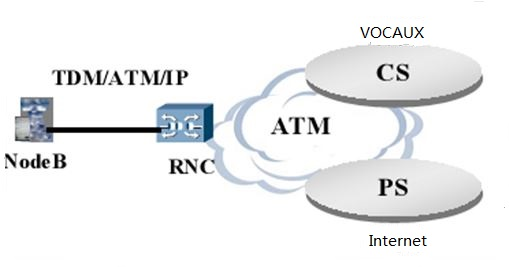
\includegraphics[width=3in]{images/3G2.JPG}}\hfill		
	\hspace{1in}
%\flushright
	\subfigure[Réseau 4G]{
		\label{Fig.3G.2}
		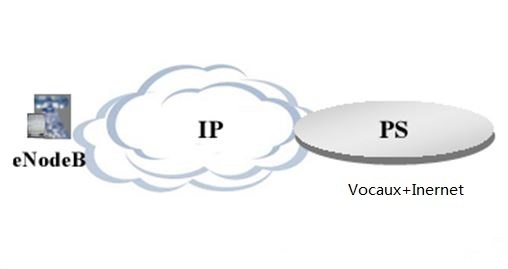
\includegraphics[width=3in]{images/4g.JPG}}
	\caption{Structure des réseaux} 
		\label{Fig.3G}
\end{figure}
Les avantages du réseau 4G sont:  plus haut débit, mieux utilisation de la bandes de fréquence, moins de délai (délai dans le panneau de l'utilisateur est inférieur que 5 ms, délai dans le panneau de commande est inférieur que 100 ms ), plus simple structure du réseau, moins de consommation d'énergie Terminal.

\subsection{Le réseau LTE}
Le LTE (Long Term Evolution) est l'evolution la plus récent des normes de CDMA 2000, TD-SCDMA, GSM. La norme LTE. La technologie LTE été considérée comme une norme de troisième génération '3.9G', et la 'vraie 4G', appelée LTE-Advanced été reconnu par l'UIT comme une technologie 4G en 2010. LTE a deux branche: LTE-FDD (Frequency-Division Duplex  Long Term Evolution)et LTE-TDD, (Time Division Duplex Long Term Evolution)les deux standards sont similaire, la différence entre les deux standard est moins de 15\% \ref{evolution}. En 2011-2012, les réseaux LTE-TDD sont commercialisés sous l'appellation 4G par le CMCC un Chine.
      \begin{figure}[H]
          \centering
          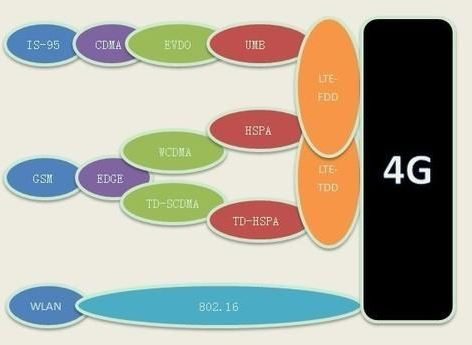
\includegraphics[width=4in]{images/evolution.JPG}
          \caption{l'evolution des standard}
          \label{evolution}
      \end{figure}
      
\subsubsection{La structure du réseau LTE}
Le réseau 4G contient 3 partie: UE( User Equipment);, eNodeB (les stations de base), EPC (Evolved Packet Core). EPC contient MME, S-GW, P-GW et HSS \ref{structure4G}  \ref{founction du chaque partie}. 
    
      \begin{figure}[H]
          \centering
          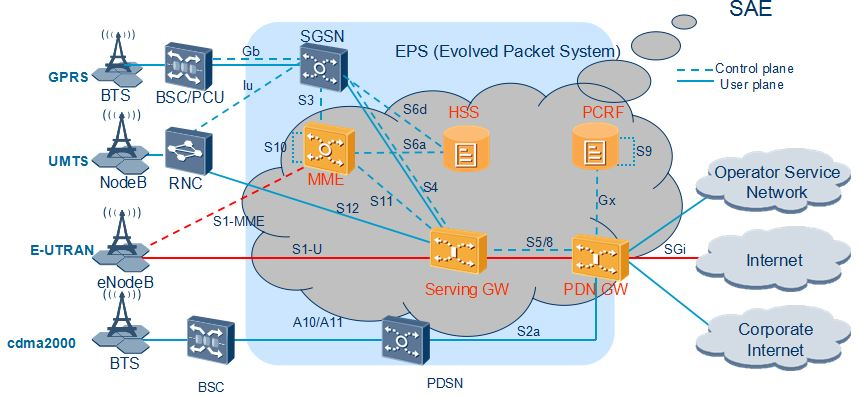
\includegraphics[width=5in]{images/enb2.jpg}
          \caption{la structure du réseau}
          \label{structure4G}
      \end{figure}
      
\begin{table}[H]
	\begin{tabular}{|>{\centering\arraybackslash}p{2cm}|>{\centering\arraybackslash}p{11 cm}|}
		\hline Part &                     Fonction\\
		\hline MME & 
			L'authentification des utilisateurs et la gestion des clés,  Cryptage de la couche NAS,  Gestion de la liste TA, Sélection P-GW ou S-GW \\ 
		\hline Service Gateway & Compression d'en-tête IP, Routage de paquets et la transmission, La commutation entre eNB, Facturation des utilisateurs porteur \\ 
		\hline PDN Gateway & L'allocation des adresses IP de UE, l'accès aux fonction de gestion de réseau externes, Facturation en service \\ 
		\hline HSS(Home Subscriber Service) & Stockée données de l'utilisateur associées au service \\ 
		\hline PCRF & Roaming \\ 
		\hline 
	\end{tabular} 
	\caption{la fonction du chaque partie}
	\label{founction du chaque partie}
\end{table}    

Entre deux \textsc{e-utran}, il y a l'interface X2, l'interface S-11 se trouve entre S-GW et MME, \textsc{e-utran} et S-GW échange les données par l'interface S1-U et il échange les donnée par l'interface S1-AP avec MME, MME et HSS utilise l'interface S6A, et l'interface S5/8 entre S-GW et P-GW, Gx entre PCRF et P-GW. En mettant des capteur en les interfaces, les opérateurs et les fournisseurs d'équipement peuvent collecter les données de signalisation, et utilisent ces informations pour trouver les défauts du système. 

\begin{figure}[H]
\centering
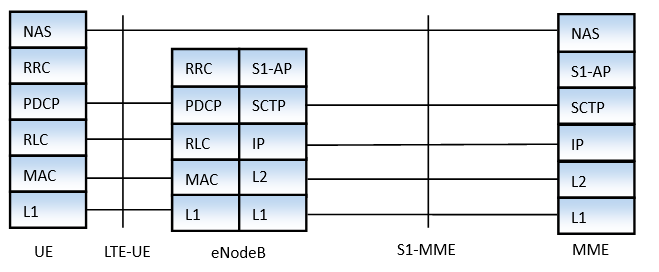
\includegraphics[width=0.9\linewidth]{images/s1-mme}
\caption{Contrôle plan}
\label{fig:s1-mme}
\end{figure}

\begin{figure}[H]
\centering
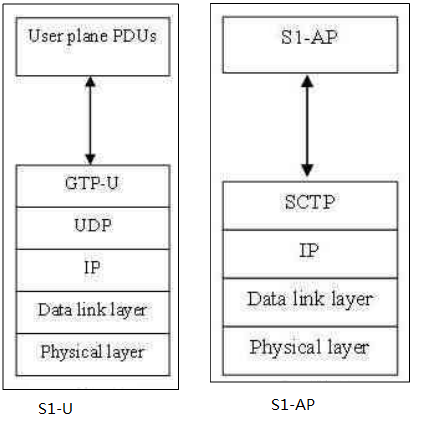
\includegraphics[width=0.9\linewidth]{images/S1-U}
\caption{User plan}
\label{fig:S1-U}
\end{figure}


\section{Les solution existant}

L'optimisation du service téléphonie est très important. L'opérateur a construit un immense réseau télécommunication, mais a cause de la mauvaise configuration du système, les utilisateur ne sont pas satisfais avec les services, les investissement n'a pas été remis. Donc les entreprises comme IBM, Huawei, et l'autre fournisseur du équipement essaient de trouver la meilleure solution. 

Maintenant, il y a beaucoup des gens travaillent sur ce domaine, nous avons trouvé beaucoup de papier sur l'optimisation du réseau télécommunication, mais les articles sont basé sur réseau 3G ou 2G. 

Il y a trois techniques qui sont beaucoup utilisé:
\begin{enumerate}
\item \textsf{la Technique KQI};
\item \textsf{la Technique QoE};
\item \textsf{la Technique qui étude les comportements de l'utilisateur}.
\end{enumerate}

\textsf{la Technique KQI}:

La technique utilise le plus souvent s'appelle 'KQI' ( Key Quality Indicator) \ref{fig:kqi}, cette méthode a été beaucoup utilisé. Et cette technique peut généralement divisé en deux étapes. d'abord, nous devons calculer le score de KPI, pour calcule le KPI en premier, il faut analyser le processus d'un service et choisir les indicateur de performances. Ensuite, nous pouvons calculer le score d'un processus en utilisant un équation linéaire, le poids de chaque attributs change selon le service, par exemple, pour le service SMS, le délai porte peu de l'importance, mais le délai du service est important pour le service HTTP. \textsf{à} la fin, nous pouvons calculer le KQI à avec les KPI \cite{kqi}. Mais les poids sont défini par les experts, et les valeurs peut-être fausse ou pas précis. Et par fois le score est bonne mais l'expérience de l'utilisateur n'est pas bon.
\begin{figure}[H]
\centering
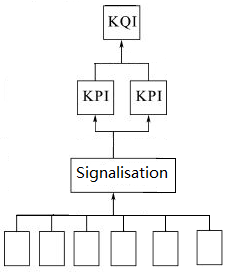
\includegraphics[width=5cm]{images/kqi}
\caption{KQI}
\label{fig:kqi}
\end{figure}

\textsf{la Technique QoE}:

KPI est un des indicateurs de qualité axés sur les performances du réseau, mais il ne reflète pas directement l'expérience de la qualité de service de l'utilisateur, parce que les expériences de l'utilisateur sont difficile à mesure. Donc la technique QoE a été inventé. QoE défini la performance, de la qualité de service et l'expérience de l'utilisateur de l'ensemble du réseau à partir de l'utilisateur.

Les utilisateurs ont nombreuses exigences pour les services téléphonie, ils peuvent être résumées comme deux aspects: la fiabilité et le confort. La fiabilité fait référence à l'activité de l'accessibilité, la disponibilité et la durabilité. Le confort est une qualité de service, est un indice de la perception directe de l'utilisateur, qui dépend à l'expérience de l'utilisateur\cite{QoE}. Les relations entre QoE et QoS KPI sont: la fiabilité du service \ref{table.fiabilité}, le confort du service\ref{table.confort}. 

\begin{table}[H]
	\centering
	\caption{Fiabilité du service }
	\label{table.fiabilité}
\begin{tabular}{|c|c|}
\hline \rule[-2ex]{0pt}{5.5ex} KQI & QoE \\ 
\hline \rule[-2ex]{0pt}{5.5ex} Accessibilité & Taux de succès  \\ 
\hline \rule[-2ex]{0pt}{5.5ex} Disponibilité  & Temps d'accès aux services \\ 
\hline \rule[-2ex]{0pt}{5.5ex} Durabilité & La durée de l'accès des services \\ 
\hline 
\end{tabular} 
\end{table}

\begin{table}[H]
	\centering
	\caption{Confort du service}
	\label{table.confort}
\begin{tabular}{|>{\centering\arraybackslash}p{5 cm}|>{\centering\arraybackslash}p{6 cm}|}
\hline KQI & QoE \\ 
\hline  & Taux de perte de paquets de couche d'application \\ 
\hline  & Le débit moyen  \newline \\ 
\hline La qualité du service de transmission & Stabilité de la transmission \\ 
\hline & Le bout en bout délai moyen \newline  \\ 
\hline & Gigue \newline  \\ 
\hline Le persistant de la connexion de service & La vitesse et la difficulté du service d'assistance\\ 
\hline 
\end{tabular} 
\end{table}

Maintenant, la technique de QoE a été beaucoup utilisé pour le service vocaux. Et grâce à la complexité du service de données, il n'y a pas un standard de QoE pour le service de données. 

En utilisant la technique KQI et QoE, nous peuvent mesurer la qualité du service, les résultats peuvent aider les opérateurs trouver les services de mauvaise qualité, les opérateur peuvent améliorer les services selon le résultat, finalement améliorer la notation de l'utilisateur.  

Le résultat de KQI dépend seulement aux performances du réseau, donc nous avons besoin les informations des performances de réseau. Et la technologie QoE besoin Le résultat de KQI et les feed-back de l'utilisateur, le feed-back peut obtenir par l'enquête ou les plaintes des utilisateurs,  et par les mesures directs.

\textsf{la Technique qui étude les comportements de l'utilisateur} 

Aussi il y a un groupe qui utilise le comportement de l'utilisateur pour défini la qualité du service\cite{UB}. Le groupe utilise cette méthode dans le service vocaux, il cherche le situation comme l'utilisateur accroche et ré-appel le même personne. \textsc{à} la fin, cette méthode aide l'opérateur corriger le paramètre d'erreur.

Selon l'article le cette méthode peut aider l'opérateur trouver les défaut du système, mais il aa nombreuses restrictions, par exemple, nous ne pouvons pas utiliser cette technologie dans le service de SMS, etc.



\section{Le présentation de notre solution}

La méthode qui utilise le comportement de l'utilisateur est intéressant, mais nous trouvons qu'elle peut utiliser seulement dans le service vocaux, nous n'avons pas trouvé les règles similaire dans l'autre service. D'ailleurs, le réseau LTE ne support pas le service vocaux, donc il n'existe pas optimisation du service vocaux dans réseau LTE et nous n'avons pas de données. Donc nous ne pouvons pas utiliser cette méthode.

La technique QoE et KQI sont beaucoup utilisé, mais d'abord, pour la méthode QoE, nous avons besoin les réponses des utilisateurs, mais nous n'avons pas assez de temps, et des raisons financières, le CMCC ne peut pas nous fournir ces données. Et le équation qu'on utilise pour calcule KPI ne sont pas convaincante, voici un exemple d'un équation pour calcule la disponibilité du réseau pour le service SMS dans réseau 3G\ref{fig:kpi}. 
\begin{figure}[H]
\centering
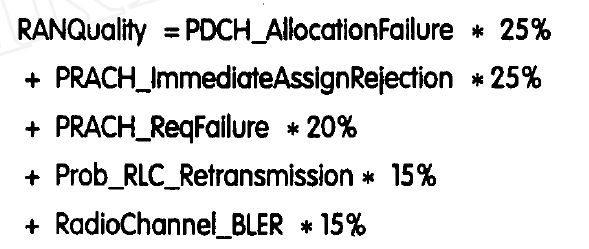
\includegraphics[width=0.7\linewidth]{images/kpi}
\caption{Un exemple d'un équation pour calculer la disponibilité}
\label{fig:kpi}
\end{figure}

Le poids du chaque attributs sont définir par les experts, Mais l'utilisateur n'est pas satisfaits du service. Nous croyons que l'erreur a été causée par l'inexacte équation, et nous pensons que les algorithmes de Classification peuvent aider à améliorer le résultat, mais très vite nous avons trouver que le CMCC ne peut pas nous fournir ce type de données. Sans le connaissance a priori, nous ne pouvons pas utiliser ces algorithmes. Nous avons aussi pense à utiliser le externalisation ouverte (crowdsourcing), à notre avis si le CMCC peut lancer un projet de externalisation ouverte, si le CMCC peut encourager ses utilisateurs donnent les note aux services pour obtenir des crédits, nous pouvons obtenir les connaissance a priori, et a l'aide de ces données, nous pouvons trouver une équation peut-être mieux que les équations écrivent par les experts. Mais bien sur, le CMCC n'a pas accepté cette idée, parce que cette méthode peut coûter cher, et peut-être il n'y a pas de revenu direct. Et l'entreprise ne fait pas de l'investissement sans retour. Donc nous n'avons pas de connaissance a priori.

Finalement, nous avons décidé d'utiliser la technique de l'apprentissage non supervisé, il contient la notion de Réseau de neurones et l'algorithme de clustering etc. Nous avons choisi l'algorithme de clustering. Et nous avons utilisé la technique de l'arbre couvrant de poids minimal en anglais Minimum spanning tree \textsf{(MST)} et la méthode \textsf{Règles d'association} et \textsf{PCA}.

\subsection{Clustering}
L'algorithme de clustering est une des méthodes de classification non supervisée. Il est beaucoup utilisé quand le donnée n'a pas de connaissance a priori.

C'est une méthodes statistiques d'analyse des données. Elle divise un ensemble de données en différents groupe, les données de chaque groupe ont mathématiquement plus proche que les données de l'autre groupe,  et nous supposons que les données dans le même partition ont des caractéristique similaires.

Il existe de multiples méthodes de regroupement des données, parmi lesquelles:
\begin{itemize}
\item Classification basées sur la densité;
\item Classification hiérarchique;
\item Classification par partitionnement;
\item Classification par grille;
\item Classification basées sur des modèles.
\end{itemize}
\vspace{1ex}

Les étapes de cette algorithme est:
\begin{itemize}
\item Choisir $k$ points qui représentent la position moyenne des $k$ partitions initiales (au hasard) ;
\item Répéter les étape suivant jusqu'à convergence :
\begin{enumerate}
\item assigner chaque observation à la partition la plus proche
\item mettre à jour la moyenne de chaque cluster
\end{enumerate}
\end{itemize}
\begin{figure}[H]
\centering
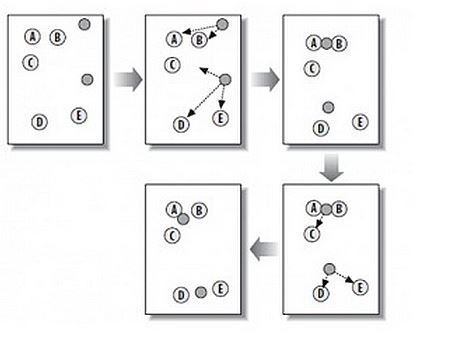
\includegraphics[width=0.7\linewidth]{images/kmeans}
\caption{étapes de l'algorithme K-Means}
\label{fig:kmeans}
\end{figure}

Nous avons utiliser l'algorithme K-Means et CLARA (Clustering Large Applications ). Ils sont deux techniques de Classification par partitionnement.

Le but de cet algorithme est de diviser des données en K partitions (clusters) dans lesquelles les données appartient à la partition avec la moyenne la plus proche. 

\subsubsection{La distance}

Quand on regroupe un ensemble de données, on calcule la distance entre chaque échantillon, la distance entre les échantillons dans un même groupe sont plus petit que les échantillons dans l'autre groupe. on suppose que les plus semblables les deux échantillons, plus la distance et petit, plus la similitude est grand.


Il y a plusieurs moyen de calculer la similarité, On utilise la technique qui basé sur la distance, les techniques utilisé le plus souvent sont: \emph{distance euclidienne}, \emph{distance de Hamming}, \emph{distance Manhattan}, etc. Aussi il existe des méthodes qui mesuré la similarité, il inclut: \emph{coefficient de Jaccard}, \emph{cosinus similarité}, etc . Nous décidons de utiliser la distance euclidienne pour calculer la similarité.

$$d(x,y) = \sqrt {\sum_{k=1}^n  (x_{k}-y_{k})^2}$$

$n$ est la dimension, $x_{k}$ et $ y_{k}$ sont le k-ème attributs de échantillon x et y.


\subsubsection{La validité de clustering}
C'est méthode a été utilisés dans beaucoup différents domaines. Mais la qualité du résultat dépend au nombre de clusters ou la valeur de K, différent paramètre peuvent mener à des résultat très différent.

En 1974, Mme \textsc{Bezdek} a proposé cette question de évaluation, et donne la première fonction pour évaluer le résultat du clustering: \textsf{Partition}  \textsf{Coefficient}. Par la suite de nombreux chercheurs ont proposé une variété de fonctions pour évaluer le résultat, et évalue les qualité et le champ d'application de ses fonctions. 

Par mesure l'efficacité entre les partitions et inter-partition, on peut évaluer le clustering. Le résultat de clustering idéal devrait être avoir la distance minimale dans le partitions, et la distance maximale entre les partitions. C'est à dire avec le plus petit grand de la cohésion dans la partition, et le plus élevé degré de la séparation entre les partitions. La cohésion mesure le degré de proximité dans la groupe, et la séparation mesure le degré de dissimilarité entre les groupe. La cohésion et la séparation peuvent calculer par les équations suivante.

$$cohésion(C_{i}) = \sum_{x\in1} proximity(x, c_{i})$$

$$séparation(C_{i},C_{j}) = proximity(c_{i}, c_{j})$$


Dans les formules, le \(c\)\ est le centre de gravité d'un partition, \(proximity(a,b)\)\ est le mesure de proximité entre la partition a et b.

Le degré de la cohésion de clusters et de la séparation est souvent utilisé comme une mesure principales pour évalue le résultat de clustering. Un bon regroupement devrait être à la fois un petit degré de la cohésion et un grand degré de la séparation.

Le degré de la cohésion et de la séparation de la partition ne sont pas indépendants, la somme des deux est une constante, on suppose que quand on a le minimal degré de la cohésion, on peut avoir le maximal degré de la séparation. \textsc{é}videment, nous devons utiliser à la fois le degré de la cohésion et de la séparation pour mesuré la qualité du regroupement.

\subsubsection{La silhouette C\oe fficient}

Kaufman a proposé la silhouette c\oe fficient en 2010, cette méthode utilise à la fois les deux degrés.

\begin{enumerate}
\item la silhouette c\oe fficient d'un échantillon:\\

 Pour un échantillon $d_{i}$, en supposent qu'il est dans groupe A, la silhouette c\oe fficient peut calculer par ce formulaire:
$$s_{i}=\frac{b_{i}-a_{i}}{max(a_{i},b_{i})} $$

\emph{$a_{i}$ est la dissemblance moyenne de la donnée i avec toutes les autres données dans le même cluster(plus la valeur est petit, meilleure est le regroupement). $b_{i}$ est la différence moyenne de $i$ à tout autre groupe $i$ n'est pas un membre.}
\vspace{1ex}

Qui peut être écrite comme:
$$  s_{i}=\left\{
\begin{array}{rcl}
1-\frac{a_{i}}{b_{i}},       &      & if\  a_{i}<b_{i}\\
0,     &      & if\ a_{i}=b_{i}\\
\frac{b_{i}}{a_{i}}-1,     &      & if\ a_{i}>b_{i}\\
\end{array} \right. $$

D'après la définition ci-dessus, il est clair que la valeur de $s_{i}$ est entre $1$ et $-1$
$$-1<s_{i}<1$$

Pour $s_{i}$ d'être proche de 1, nous demandons le $a_{i}$ plus petit que $b_{i}$. Comme $a_{i}$ mesure la dissemblable de i et son propre groupe, une petit valeur signifie qu'il est bien adapté. En outre, un grand $b_{i}$ implique que i est mal adapté à son groupe voisin. Ainsi, un $s_{i}$ près de $1$ signifie que la donnée est concentrée de manière appropriée. Si la valeur de $s_{i}$ est proche de $-1$, selon la même logique, nous voyons que le donnée $i$ serait plus approprié si elle a été regroupée dans son groupe voisin.

\item la silhouette c\oe fficient moyenne:

Pour le résultat d'un regroupement, le silhouette c\oe fficient égale à:
$$s_{k}=\frac{1}{n}\sum_{i=1}^n s_{i}$$
\emph{$n$ est le nombre de données, $k$ est le nombre de partition, $s_{k}$ est la moyenne du silhouette c\oe fficient. Nous pouvons utiliser $s_{k}$ pour évalue la qualité du clustering.}
\newline
\newline
Le $s_{i}$ est les moyens sur l'ensemble des données d'un cluster, il est un mesure le degré de cohésion de toutes les données du cluster. Ainsi, les moyens de $s_{i}$ de l'ensemble des données ($s_{k}$) est une mesure de la façon appropriée les données ont été regroupés. S'il y a trop peu de clusters, ainsi que peut se produire lorsque un mauvais choix de k est utilisé dans l'algorithme K-Means, la silhouette C\oe fficient de certains groupes est beaucoup plus petit que les autres. Donc la plot de silhouette C\oe fficient et la valeur moyenne de silhouette peuvent être utilisé pour déterminer le nombre de cluster (la valeur de $k$ ) optimal pour le ensemble de données.
\end{enumerate} 

Après trouver les paramètre optimal, nous pouvons utiliser l'algorithme clustering, et après étudié et comparé les caractéristiques de chaque partition, on pouvons défini quelle partition représentent mauvais qualité de service. Les résultat peut nous aider à classifier le service. 

\subsection{Règles d'association}
La règle d'association est une méthode populaire, elle étudiée d'une manière approfondie dont le but est de découvrir des relations ayant un intérêt pour le statisticien entre les variables. En se basant sur le concept de relations fortes, Rakesh Agrawal et son équipe présente des règles d'association dont le but est de découvrir des similitudes entre des produits dans des données saisies sur une grande échelle dans les systèmes informatiques des points de ventes des chaînes de supermarchés. Par exemple, une règle découverte que si un homme achète les serviettes de bébé, il est susceptible de achète les bières. Une telle information peut être utile quand on veut prendre des décisions marketing.

Les règles d'association sont employées aujourd'hui dans plusieurs domaines, incluant: la fouille du web, la détection d'intrusion et la bio-informatique.  Dans ces domaines, ils utilisent les données booléenne pour trouver les règles utiles. Mais dans le domaine télécommunication, les données de signalisation sont le données numérique. Donc nous ne pouvons pas directement utiliser la règles d'association. Par contre nous pouvons convertir les données de type numérique en données de caractère en divisant les données dans plusieurs partitions \cite{AR}. Par exemple, nous avons des données numérique entre $0$ et $100$, et on divise les données en 10 partitions, donc les chiffres entre $0$ et $10$ peuvent présenter par $0<x<10$. En utilisant cette technique nous pouvons utiliser la règle d'association pour trouver les relations dans les données.

 Il y a plusieurs méthodes pour diviser les attributs numériques: par catégorisation, l'analyse typologique, par analyse de l'histogramme, l'analyse basé sur l'entropie de discret, partition naturel et ainsi de suite. 
 
 Nous décidons de utiliser le K-Means d'abord. Après analyse le résultat, nous pouvons utiliser la algorithme règles d'associations à l'aide du résultat de K-Means.

\subsection{K-Means et l'arbre couvrant de poids minimal }
D'après les techniques précédant, nous avons utilisé l'arbre couvrant de poids minimal avec K-Means.

En théorie des graphes, étant donné un graphe non orienté connexe dont les arêtes sont pondérées, un arbre couvrant de poids minimal de ce graphe est un arbre couvrant (sous-ensemble qui est un arbre et qui connecte tous les sommets ensemble) dont la somme des poids des arêtes est minimale\ref{fig:mst}. L'arbre couvrant de poids minimal est aussi connu sous certains autres noms, tel qu'arbre couvrant minimum ou encore arbre sous-tendant minimum. L'algorithme de Prim et l'algorithme de Kruskal sont deux méthodes classique, qui sont tous les deux l'algorithme glouton. 

\begin{figure}[H]
\centering
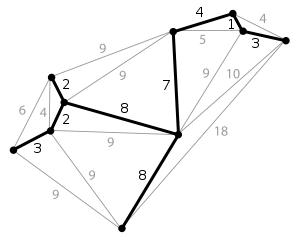
\includegraphics[width=0.5\linewidth]{images/mst}
\caption{MST}
\label{fig:mst}
\end{figure}

En coupant $C-1$ arêtes le plus grand, nous pouvons grouper le données en $C$ parties.
\begin{figure}[H]
\centering
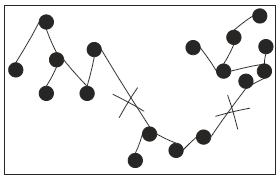
\includegraphics[width=0.4\linewidth]{images/mstc}
\caption{MST clustering}
\label{fig:mstc}
\end{figure}

Dans notre projet, nous avons choisi l'algorithme Prim et K-Means pour faire le clustering. 

La complexité de algorithme Prim est: $O((V+E)+\lg (V) = O(E \lg (V)) $, $V$ est l'ensemble de vertex ,$E$ est l'ensemble de arêtes.

la complexité de algorithme K-Means est: $O(nkt)$, $n$ est la quantité de données, $k$ est le nombre de partitions, t est le nombre d'itérations.
\subsubsection{L'algorithme KmMST}

Dans l'article \cite{KmMst}, nous avons trouvé une algorithme qui utilise K-Means et la MST. 

Parce que K-Means peut trouver des partitions sur forme sphéricité, et la valeur de $K$ n'est pas grand donc le résultat est influencer par les donnée de bruits, donc le résultat de K-Means est par fois peu satisfaisant. 

D'après l'article, nous pouvons choisir une grand valeur pour K, plus utilise la technique MST pour combiner les partition en C groupes en coupant C-1 arête. La performance est mieux que celui de K-Means\ref{fig:kmmst}.
\begin{figure}[H]
\centering
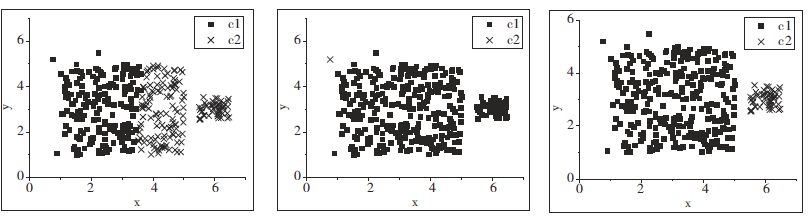
\includegraphics[width=1.0\linewidth]{images/kmmst}
\caption{La performance de K-Means, MST et KmMST}
\label{fig:kmmst}
\end{figure}

L'algorithme KmMST peut décrire comme suit:
Input: le données de quantité $n$, c\oe fficient $r$ et $C$.
output: les partitions.
l'étape:
\begin{enumerate}
\item calcule la valeur de $K$, $k=\left\vert n^r \right\vert \quad  \left( r \in \left[ 0,1 \right]  \right) $ par défaut la valeur de $r$ égale à $0,5$;
\item utilise l'algorithme K-Means, trouve K partitions;
\item calcule la distance entre chaque centre de la partition;
\item utilise l'algorithme Prim pour crée l'arbre couvrant de poids minimal;
\item coupe le $C-1$ plus bords qui ont le plus grand distance, le $C$ sous-graphe est le résultat de clustering.
\end{enumerate}

\section{La mise en \oe uvre}
\subsection{Le logiciel utilisés}
L'objectif de notre projet est de trouver une méthode qui peut s'implanter dans les serveurs du CMCC, et aider le CMCC améliorer la qualité du réseau. D'après le directeur du R\&D département du CMCC, au total, il a $20Pb$ de donnée stock dans ses base de données, donc le logiciel doit être capable d'exécuter grand quantité de données. En plus,  au lieu de utilisé directement les logiciel comme SQL (qui n'est pas très efficient si on a beaucoup de donnée stock dans différent serveur), le CMCC utilise 'Hadoop' pour stock et géré ses données.

Donc le logiciel que nous utilisons doit être capable d'exécuter grand quantité de donnée et peut travailler avec Hadoop. 

Finalement nous décidons de utiliser le langage \textsf{R}. L'avantage de R sont:

\begin{itemize}
\item R est un langage et un environnement pour le calcule statique et les graphiques; 
\item R offre une grande variété de statistiques (modélisation linéaire et non linéaire, classification, clustering, etc,) et des graphiques techniques, et il est très extensible ;
\item R est facile à utiliser; 
\item R est un logiciel libre, il compile et fonctionne sur une grande variété de plates-formes UNIX et les systèmes similaires (y compris FreeBSD et Linux), Windows et Mac OS;
\item en utilisant les packages fournir par 'Revolution Analytics', nous pouvons utiliser Hadoop en R.
\end{itemize}

Nous utilisons \textsf{Rstudio} comme notre environnement de programmation. C'est une interface utilisateur puissante et productive pour R.

\subsection{Introduction des données}
%\,\up{\cite{specifi}}
Après quelque semaines de négociation avec les employés de différents départements de le CMCC, ils nous ont fourni deux versions de données, et ses spécifications du format\cite{specifi}. Nous avons trouvé que le CMCC n'a pas de accès direct aux données, et le fournisseur d'équipement a modifié le spécification fournir par le CMCC, et il y a des erreurs dans les données fourni par les fournisseur d'équipement.

Ils nous ont envoyé $11$ dossiers, chaque dossier correspond à un service. les services sont 'rtsp', 'dns','mail', 'ftp', 'http-wap', 'mms', 'p2p', 'realtimecom', 'VoIP' et les données de signalisation entre \textsc{e-utran} et MME 'S1AP-NAS'.
    
Et nous avons trouvé que pour les services comme 'VoIP' et 'RTSP', ils sont très peu de données \ref{table.nombre}. Donc nous avons décidé de utiliser le donnée du service 'HTTP'.

\begin{table}[H]
\centering
	\begin{tabular}{|>{\centering\arraybackslash}p{4 cm}|>{\centering\arraybackslash}p{4 cm}|}
	\hline \textsf{L'interface }& \textsf{Nombre de ligne} \\ 
	\hline S1-AP & $240$ \\ 
	\hline RTSP &$ 35$ \\ 
	\hline DNS  & $272562$ \\ 
	\hline Maill & $44$ \\ 
	\hline FTP &$ 71$ \\ 
	\hline HTTP-WAP & $50854$ \\ 
	\hline MMS & $193$ \\ 
	\hline P2P & $515$ \\ 
	\hline Realtimecom & $2082$ \\ 
	\hline S1U &$ 89759$ \\ 
	\hline VoIP & $28$ \\ 
	\hline 
	\end{tabular} 
	\caption{les dossiers de données}
	          \label{table.nombre}
\end{table}


Le dossier du service HTTP a $18,4Mbit$ , il y a $50854$ lignes, tous les données sont collectées par les capteurs placer entre les Service-Gateway et les eNodeB. le capteur enregistre un ligne de donnée quand un processus est fini. chaque ligne a $76$ attributs\ref{Fig.HTTP}.

      \begin{figure}[H]
          \centering
          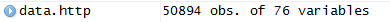
\includegraphics[width=3.5in]{images/http.png}
          \caption{les données du service HTTP}
          \label{Fig.HTTP}
      \end{figure}
      
Il contient des informations de UE (IMEI, IMSI, etc), les trafic de la liaison montante et la liaison descendante et le temps, la adresse IP de UE, eNodeB et S-GW, le port de UE, eNodeB et S-GW, le délai du service, le site web, cookie, et aussi le début temps et le temps d'arrêter.
les données sont collectent dans $20.92$ minutes \Ref{fig:lasttime}.

      
      \begin{figure}[H]
\centering
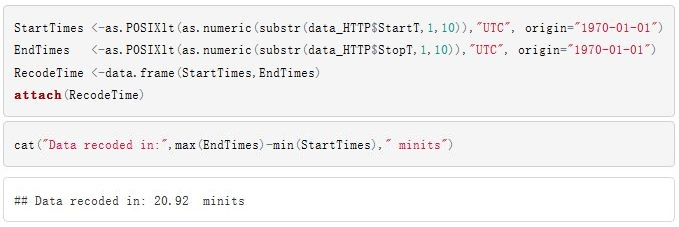
\includegraphics[width=15Cm]{images/lasttime}
\caption{Les données sont collectent dans 20.92 minutes}
\label{fig:lasttime}
\end{figure}

\subsection{Prétraitement de données}
En analysant des données, nous avons trouvé des erreurs de données, et le fournisseur nous a confirmé que ces sont les défaut de leur système 4G. Pour les attributs 'IMSI', 'IMEI', 'MSISDN', $90$ \% de lignes sont vides, ce qui ne sont pas vides, les contenus sont illisible, et peuvent provoquant des erreurs de lecture \ref{fig:errorData}. Et nous avons trouvé que dans les contenus de certains lignes sont bizarre. 
\begin{figure}[H]
	\centering
	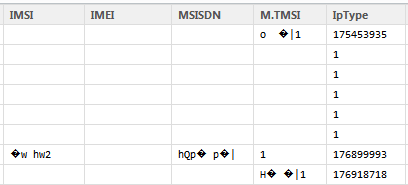
\includegraphics[width=0.7\linewidth]{images/errorData}
	\caption{erreur du codage BCD}
	\label{fig:errorData}
\end{figure}
Dans ce processus, le 'Down Link Online Time' égale à  $0$ ms , mais il a téléchargé $746$ bits, c'est clairement un erreur du données.
\begin{figure}[H]
	\centering
	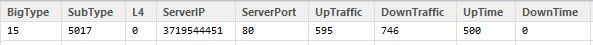
\includegraphics[width=0.9\linewidth]{images/bizarre}
	\caption{Erreur de la donnée}
	\label{fig:bizarre}
\end{figure}

 Nous avons décidé de ne utiliser les données avec ce type de erreur, à la fin, en supprimant ses données, il nous reste $37865$ lignes ($50894$ lignes en origine, $13029$ lignes ont été supprimé)  \ref{fig:newdata}.
 
\begin{figure}[H]
	\centering
	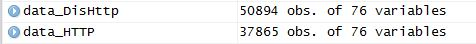
\includegraphics[width=0.8\linewidth]{images/newdata}
	\caption{Prétraitement des données}
	\label{fig:newdata}
\end{figure}

Entre ces 76 attributs, Une grande partie de ces informations sont inutile, et pour certain attributs les contenus égal tous à 0. Finalement nous avons trouvé 11 attributs. ils sont:
\begin{table}[H]
\centering
\begin{tabular}{|>{\centering\arraybackslash}p{3 cm}|>{\centering\arraybackslash}p{3 cm}|>{\centering\arraybackslash}p{3 cm}|}
\hline \rule[-2ex]{0pt}{5.5ex} Signalisation & Signalisation & KPI \\ 
\hline \rule[-2ex]{0pt}{5.5ex} trafic en liaison montante & le temps en ligne & vitesse \\ 
\hline \rule[-2ex]{0pt}{5.5ex} trafic en liaison descendante  & le temps en ligne & vitesse \\ 
\hline \rule[-2ex]{0pt}{5.5ex}  & Http First Response Time & délai \\ 
\hline \rule[-2ex]{0pt}{5.5ex}  & Http Last Packet Time & délai \\ 
\hline \rule[-2ex]{0pt}{5.5ex}  & Http Last Ack Time & délai \\ 
\hline \rule[-2ex]{0pt}{5.5ex}  Packet Num en liaison montante & retransmission de paquets Num en liaison montante & taux de retransmission \\ 
\hline \rule[-2ex]{0pt}{5.5ex}  Packet Num en liaison descendante & retransmission de paquets Num en liaison descendante& taux de retransmission \\ 
\hline 
\end{tabular} 
\end{table}


Mais nous avons trouvé que dans certains lignes le taux de retransmission sont trop grands ( plus grand que $100\%$). par exemple, dans un processus, il a téléchargé  $17$ paquets IP, et il a  $7448$  paquets sont désordre, et  ré-téléchargé  $6384$ paquets  \ref{fig:défaut}. Les données ne sont pas correct, donc nous ne pouvons pas utiliser ses donnée pour calculer le taux de retransmission.  
\begin{figure}[H]
	\centering
	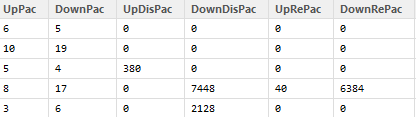
\includegraphics[width=0.7\linewidth]{images/11}
	\caption{Défaut de la système}
	\label{fig:défaut}
\end{figure}

Finalement nous avons décidé de utiliser ces 5 attributs (la vitesse et le délai) pour mesurer la qualité du service.

\subsection{Les caractéristique du donnée}



\begin{figure}[H]
\centering
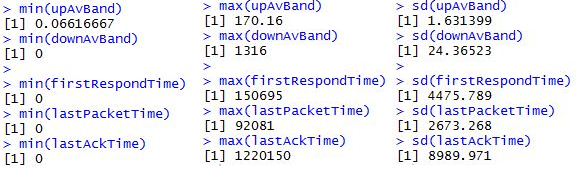
\includegraphics[width=0.8\linewidth, height=0.2\textheight]{images/max-min}
\caption{La valeur maximal, valeur minimal et l'écart type}
\label{fig:max-min}
\end{figure}

\begin{figure}[H]
\centering
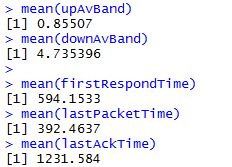
\includegraphics[width=0.3\linewidth]{images/mean}
\caption{La valeur moyenne}
\label{fig:mean}
\end{figure}

Nous avons trouvé que l'écart type pour les trois attributs de délais sont très grand. Les valeurs varient de $0ms$ à $1220150ms$. Par contre la changement  de la vitesse de la liaison montante et descendante n'est pas très grand.

\begin{figure}[H]
\centering
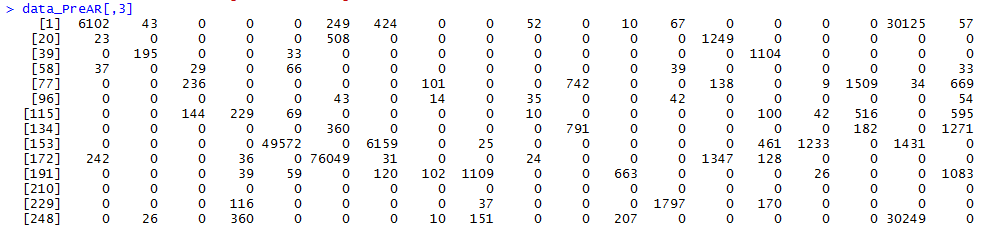
\includegraphics[width=0.9\linewidth]{images/data-delai}
\caption{Le temps de réponse du serveur}
\label{fig:data-delai}
\end{figure}
En analysant le données, nous avons trouvé que les données ne sont pas normal, et l'ingénieur du fournisseur de l'équipement nous ont confirmé que le système de collecte d'informations de signalisation a des défauts. 
 
%\section{La mise en \oe uvre}
\subsection{Le K-Means et Le Règle d'association }
\subsubsection{La valeur optimal de $k$}
Pour trouvé le k optimal pour notre données, nous avons utilisé la technique 'silhouette C\oe fficient' et 'somme de erreur carrés'.

Nous avons mesuré le résultat de ces deux techniques quand la valeur de $k$ augmente de $1$ à $15$, étant donné que les caractéristique de l'algorithme, pour chaque valeur de $k$, nous avons répétées 50 fois et calcule la valeur moyenne pour éliminer les erreurs, en suite, nous étudions le résultat pour trouver la valeur optimal.
\subsubsection*{La somme d'erreur carrés}
\begin{figure}[H]
\centering
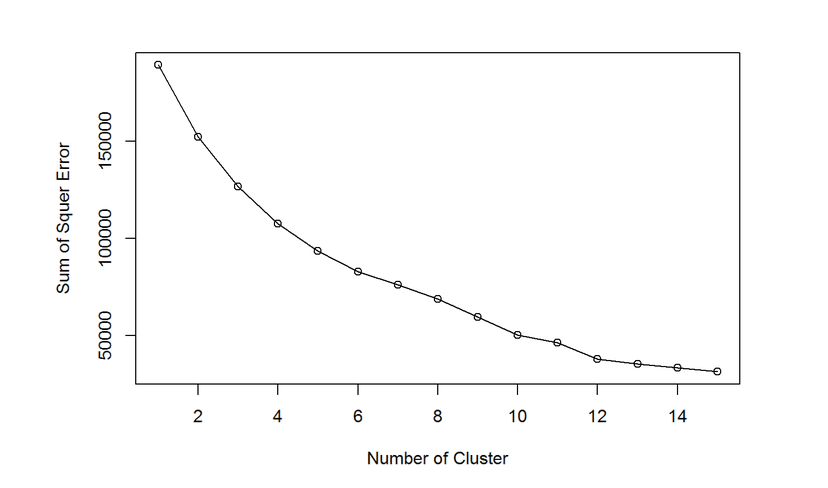
\includegraphics[width=0.8\linewidth]{images/sse}
\caption{somme d'erreur carrés}
\label{fig:sse}
\end{figure}
Nous avons trouvé que la somme d'erreur carrés diminue quand $k$ augment, mais il est difficile de choisir la valeur optimal de $k$ avec cette image.

\subsubsection*{La silhouette C\oe fficient}
Nous utilisons la même technique pour calculer et visualiser la valeur de la silhouette C\oe fficient.

\begin{figure}[H]
\centering
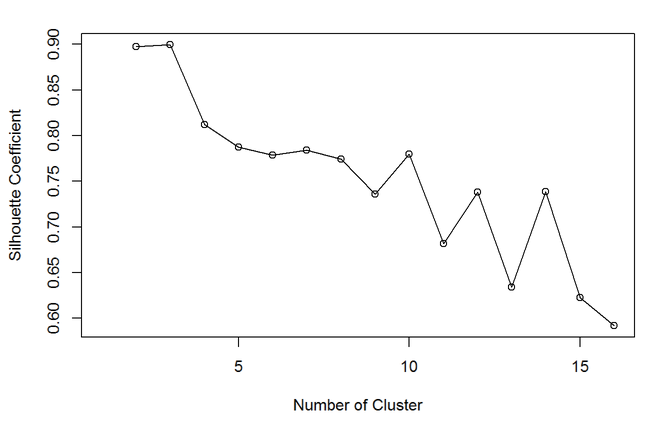
\includegraphics[width=0.9\linewidth]{images/sc}
\caption{la silhouette C\oe fficient quand k varie de 2 à 15}
\label{fig:sc}
\end{figure}

L'image de la silhouette C\oe fficient nous montrons que comme quand $k=3$ la valeur de la silhouette C\oe fficient est plus grand. Donc nous soupçonnons que quand $k=3$ nous pouvons trouver le mieux partition.

\subsubsection{Le clustering}
Après classifie le données en 3 groupes utilisant l'algorithme CLARA. Nous avons trouvé que la majorité de données ($94 \%$ de données) sont dans le premier groupe, un groupe de $4,4 \%$, la troisième groupe a $1,6 \%$ de données.  

 \begin{figure}[H]
 	\flushleft
 	 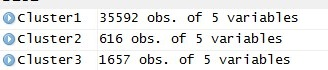
\includegraphics[width=0.45\linewidth]{images/3cluster}
 	 \label{fig:3cluster}
 	\hspace{1in}	 
 	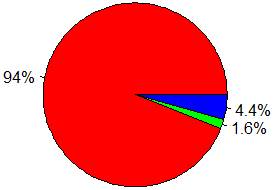
\includegraphics[width=0.325\linewidth]{images/piechart}
 	\label{fig:piechart}
 	\caption{Cluster} 
 \end{figure}

En utilisant le fonction 'plot3d' fourni par le package 'rgl', nous pouvons visualiser le données en trois dimensions, et nous pouvons visualiser le résultat de clustering.


% bande passante moyenne de la liaison montante, bande passante moyenne de la liaison descendant, et le premier délai de réponse
\begin{figure}[H]
\centering
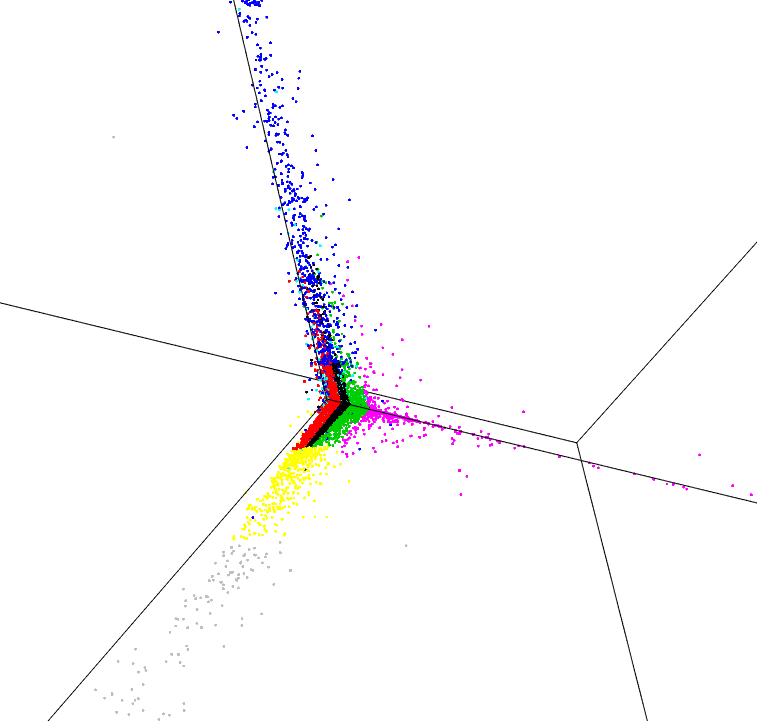
\includegraphics[width=0.6\linewidth]{images/kmeqn}
\caption{up link Average Band, down link Average Band, first Respond Time.}
\label{fig:kmeqn}
\end{figure}
\begin{figure}[H]
\centering
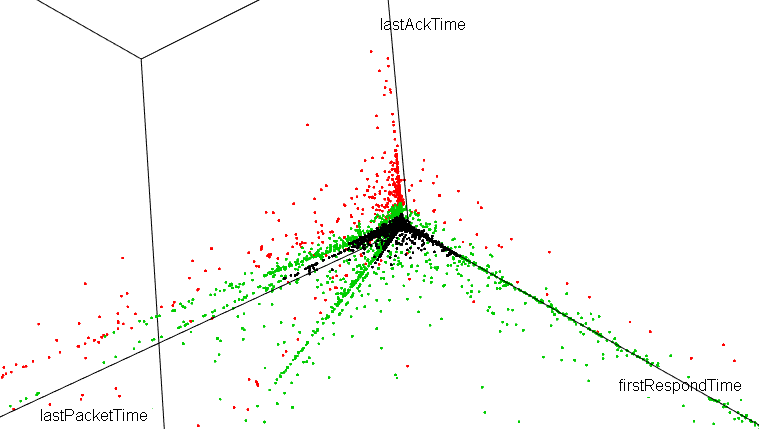
\includegraphics[width=0.8\linewidth]{images/3delai}
\caption{first Respond Time, last Packet Time, last Ack Time.}
\label{fig:3delai}
\end{figure}

Nous avons trouver que le données de 'cluster 1' sont les points sont colorent en noir, 'cluster 2' en rouge, 'cluster 3' en vert. 

Après le regroupement, nous pouvons utiliser l'algorithme 'k plus proches voisins' pour déterminer le nouveau données font partie de quel groupe .

\subsubsection{Le Règle d'association}
En utilisant le résultat de clustering, nous pouvons transformer les données numérique à données caractère. 

Nous y parvenons en quatre étapes
\begin{enumerate}
\item D'abord, nous avons trouvé les valeur minimal et maximal de chaque attribut\ref{fig:max-min1};
\item Ensuite, nous avons trouvé les intervalles de chaque attribut\ref{fig:seuil};
\item Puis, nous avons transformé les données numérique à données caractère\ref{fig:newData2};
\item \textsc{à} la fin, nous avons utilisé l'algorithme Apriori pour trouver des règles\ref{fig:newar}. 
\end{enumerate}
\begin{figure}[H]
\centering
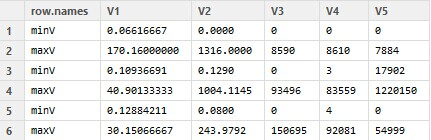
\includegraphics[width=0.8\linewidth]{images/max-min1}
\caption{trouver les valeur minimal et maximal de chaque attribut}
\label{fig:max-min1}
\end{figure}


\begin{figure}[H]
\centering
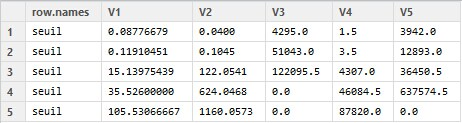
\includegraphics[width=0.8\linewidth]{images/seuil}
\caption{défini les intervalles}
\label{fig:seuil}
\end{figure}

\begin{figure}[H]
\centering
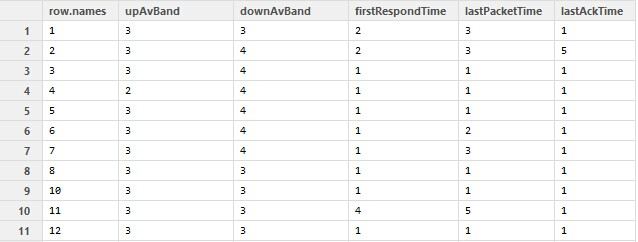
\includegraphics[width=0.8\linewidth]{images/newData2}
\caption{transformer les données numérique à données caractère}
\label{fig:newData2}
\end{figure}

\begin{figure}[H]
\centering
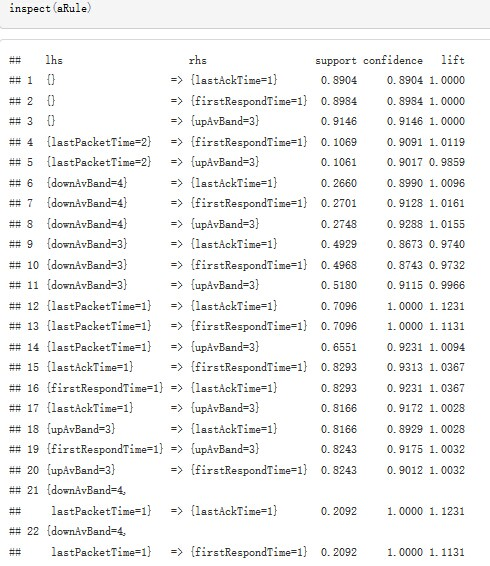
\includegraphics[width=0.8\linewidth]{images/newar}
\caption{Les règles été trouvé par l'algorithme règle d'association  }
\label{fig:newar}
\end{figure}

\subsection{Le KmMST}
 Par clustering le données en beaucoup de partitions, et utilise la technique de MST, nous pouvons surmonter les défaut de K-Means et clustering le données..
 
  \subsubsection{L'étape de l'algorithme KmMST}
  
  \begin{enumerate}
  \item Regroupement le données;\\
  
   La valeur de $K$ égal à $n^r$, le $n$ égal à la quantité de données, $r$ est dans l'intervalle de $0$ et $1$, par défaut, $r$ égal à $0,5$.
   
   En premier, nous avons regroupé le données en K partition.
   
  \item \textsc{é}tablir la matrice de distance;\\
  
  Après, nous pouvons utiliser les valeurs du centre de chaque partition pour calculer la matrice de distance
  \begin{figure}[H]
\centering
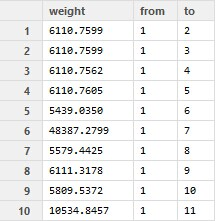
\includegraphics[width=0.4\linewidth]{images/distance}
\caption{la matrice de distance}
\label{fig:distance}
\end{figure}

  
  \item Utilise la technique de MST;\\
  
  \textsc{à} aide de la package 'igraph' nous pouvons trouver l'arbre couvrant de poids minimal.
  
  \begin{figure}[H]
\centering
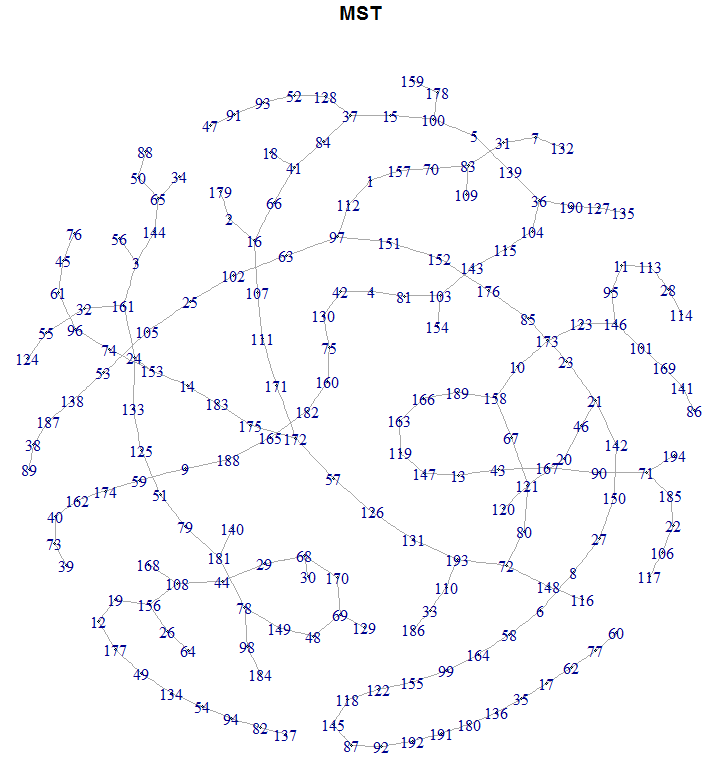
\includegraphics[width=0.45\linewidth]{images/mst2}
\caption{L'arbre couvrant de poids minimal}
\label{fig:mst2}
\end{figure}

  \item Coupe le arête le plus long
  
  Techniquement, nous pouvons trouver les partitions par couper les arête long, et nous avons tester avec différentes valeurs, mais les sommets sont devenu le point isolé.
  
  \begin{figure}[H]
\centering
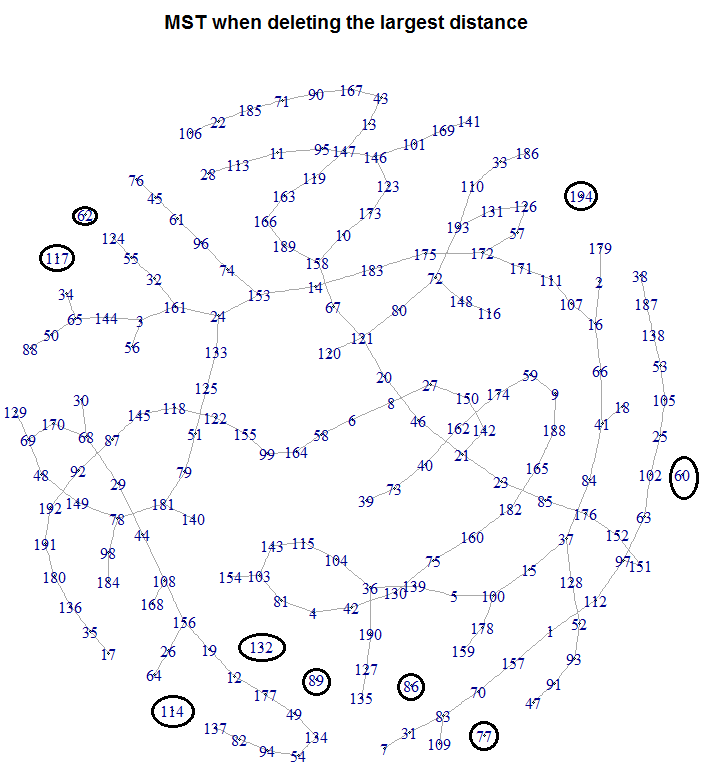
\includegraphics[width=0.6\linewidth]{images/mst10}
\caption{L'arbre couvrant de poids minimal, quand C = $10$}
\label{fig:mst10}
\end{figure}

  \end{enumerate}








